%# -*- coding: utf-8-unix -*-
% !TEX program = xelatex
% !TEX root = ../thesis.tex
% !TEX encoding = UTF-8 Unicode
%%==================================================
%% chapter01.tex for SJTU Master Thesis
%%==================================================

%\bibliographystyle{sjtu2}%[此处用于每章都生产参考文献]

\newcommand{\bodyframe}{\left\{ \mathbf{b} \right\}}
\newcommand{\NEDframe}{\left\{ \mathbf{n} \right\} }

\chapter{船体运动模型}
\label{chap:chapter01}

本章介绍船体运动模型,主要分为单自由首要控制模型、3自由度操纵性模型、3自由度动力定位模型、
4自由度带有横摇补偿的操纵性模型。

\section{坐标系}
\subsection{北东地坐标系}
北东地(North-East-Down: NED)坐标系$\NEDframe=(x_n, y_n, z_n)$是
常用的导航坐标系,通常定义在地球表面的切平面上,其中$x$轴指向地球北,$y$轴指向地球东,
$z$轴垂直于地球表面并指向下。通常对于海上船舶,经纬度的变化并不大,我们可以假定$\NEDframe$
是惯性参考系。

北东地坐标系在程序里也称Marine coordinate,与之对应的是UTM坐标系
(UTM-x指向正东,UTM-y指向正北)。

\subsection{笛卡尔坐标系}
笛卡尔(Cartesian)坐标系如图\ref{fig:3Dcartesian}在数学中是一种正交坐标系,
由法国数学家勒内·笛卡尔引入而有此名。二维的直角坐标系是由两条相互垂直、
相交于原点的数线构成的。在平面内,任何一点的坐标是根据数轴上对应的点的坐标设定的。
在平面内,任何一点与坐标的对应关系,类似于数轴上点与坐标的对应关系。

\subsection{随体坐标系}
随体坐标系 $\bodyframe$ 始终跟随船体的运动,通常我们随体坐标系的原点$o_b$置于船体中轴线上,
并位于船尾甲板处(船体上比较容易接触到某一点)。
一般我们用六个变量来描述船体的运动,主要分为平动($x,y,z$)和转动($\phi, \theta, \psi$),
具体的描述和符号见图\ref{fig:Coordinate}和表\ref{tab:notation}。图中,CoG在随体坐标系
中相对于$o_b$的坐标可表示为$\mathbf{r}_g = (x_g,y_g, z_g)^T$

\begin{figure}[!htp]
  \centering
  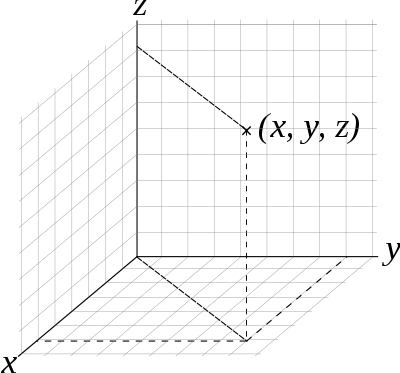
\includegraphics[width=9cm]{chapter01/3D_Cartesian.png}
  \bicaption[笛卡尔坐标系]
    {笛卡尔坐标系}
    {Cartesian coordinate system}
  \label{fig:3Dcartesian}
\end{figure}

\begin{figure}[!htp]
  \centering
  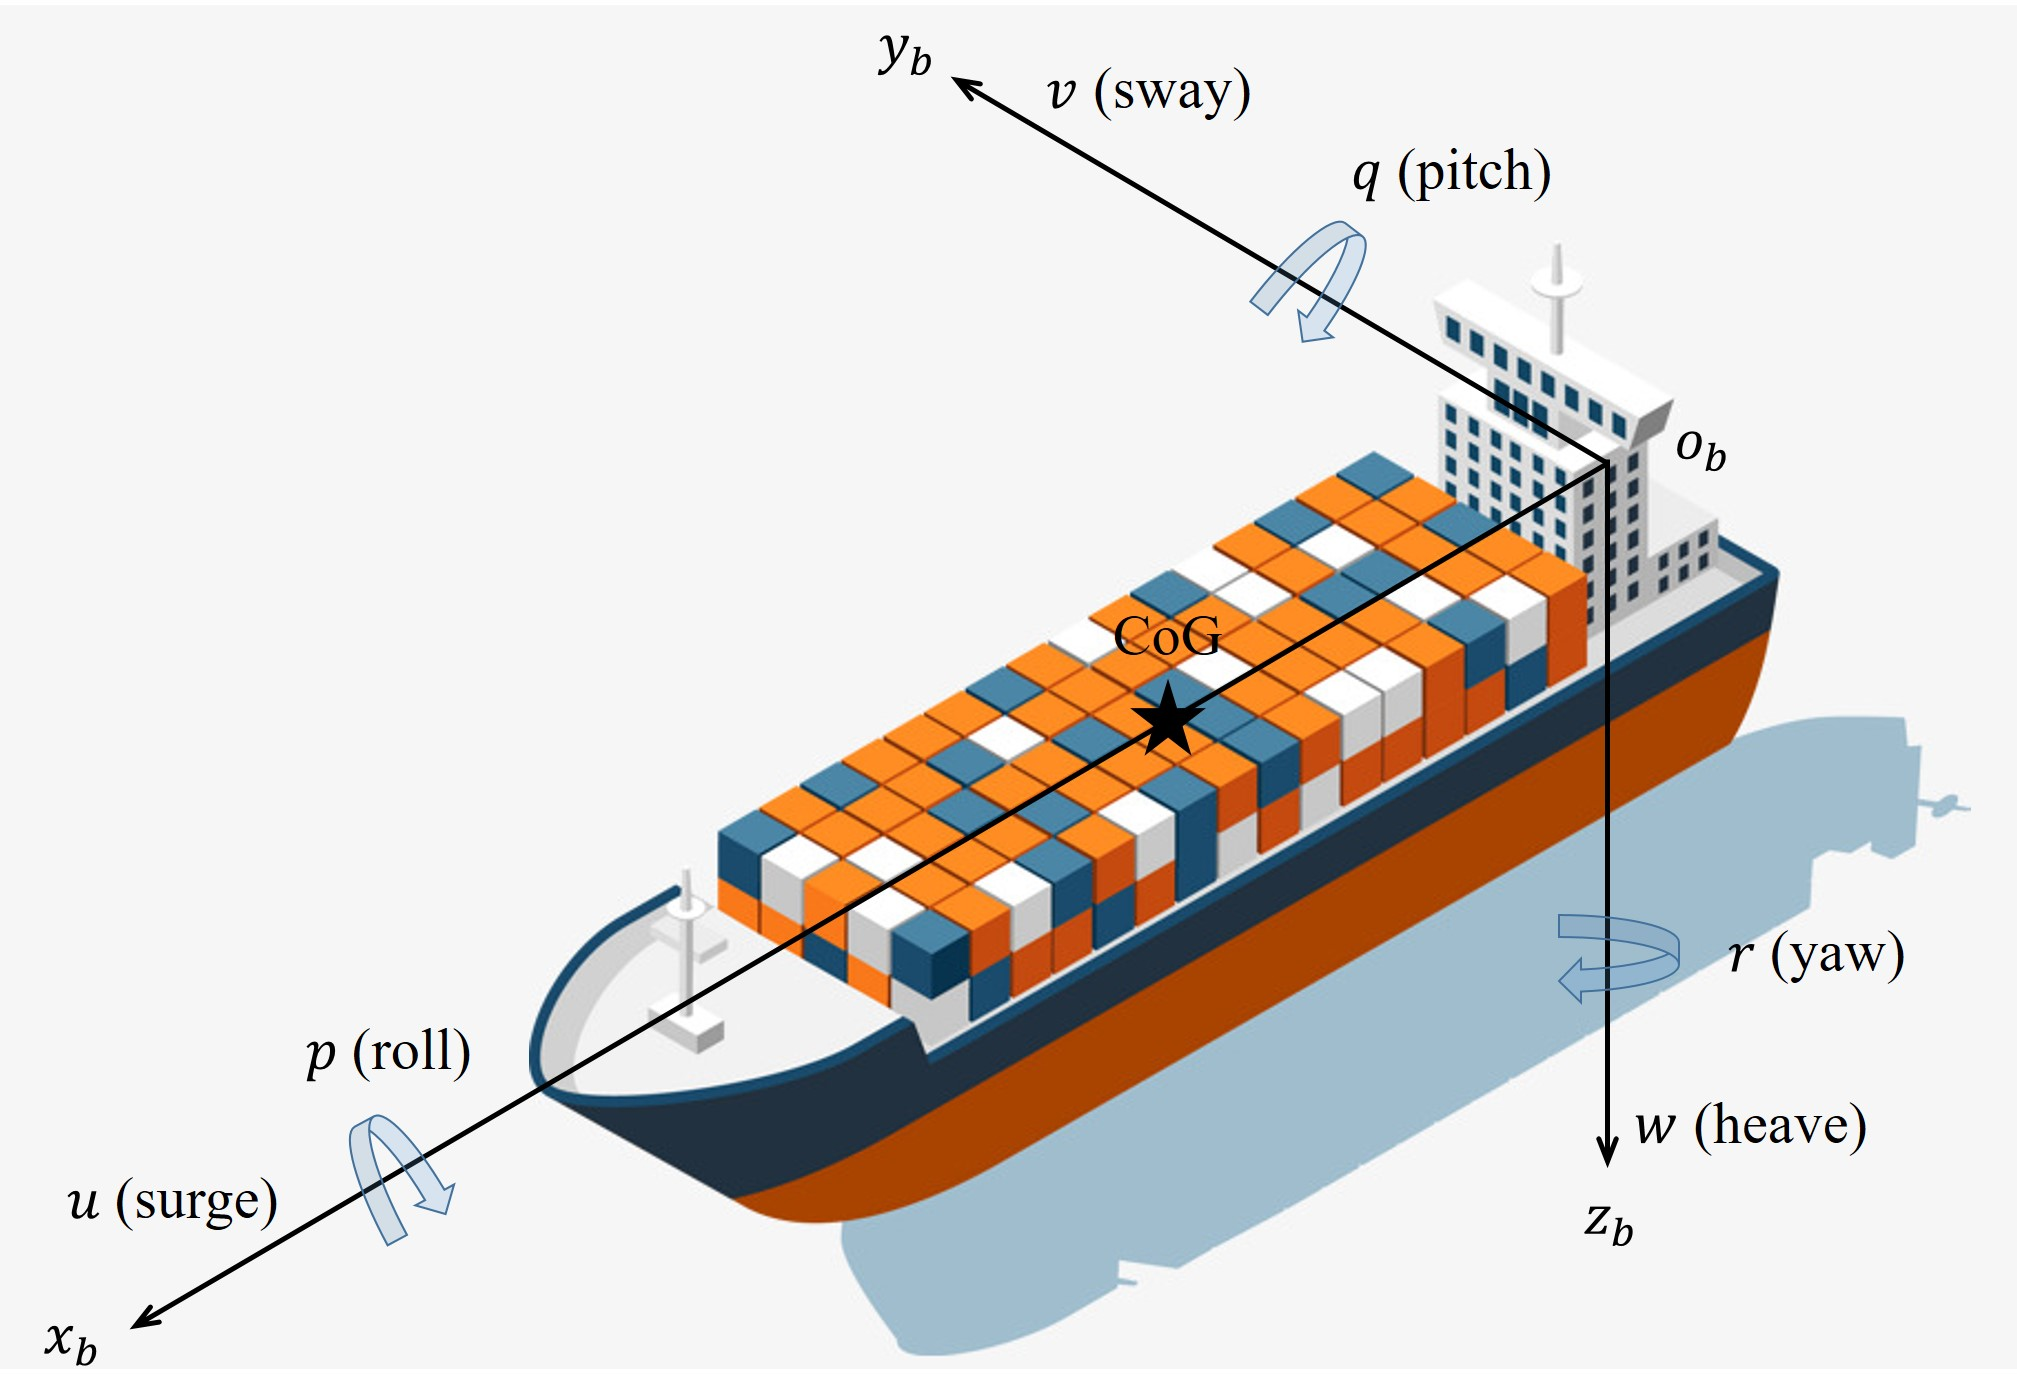
\includegraphics[width=13cm]{chapter01/Coordinate.jpg}
  \bicaption[在随体坐标系中,船体六自由度的速度 $u,v,w,p,q,r$]
    {在随体坐标系 $\bodyframe$ 中,船体六自由度的速度 $u,v,w,p,q,r$}
    {The 6DoF velocities $u,v,w,p,q,r$ in the body-fixed reference frame
    $\bodyframe=(x_b, y_b, z_b)$  }
  \label{fig:Coordinate}
\end{figure}


% Table generated by Excel2LaTeX from sheet 'Sheet1'
\begin{table}[htbp]
  \centering
  \caption{描述船体运动的常用符号}
    \begin{tabular}{llll}
    \toprule
    自由度(DOF) & 力/力矩  & 线/角速度 & 位置/欧拉角 \\
    \midrule
    1 \quad surge & $X$     & $u$     & $x$ \\
    2 \quad sway &  $Y$     & $v$     & $y$ \\
    3 \quad heave & $Z$     & $w$     & $z$ \\
    4 \quad roll & $K$     &  $p$     & $\phi$ \\
    5 \quad pitch & $M$     & $q$     & $\theta$ \\
    6 \quad yaw & $N$     &   $r$     & $\psi$ \\
    \bottomrule
    \end{tabular}%
  \label{tab:notation}%
\end{table}%

\subsection{运动方程}


\section{海洋环境载荷}
风、浪、流


\section{三自由度操纵性方程}
三自由度操纵性方程只考虑低频的surge, sway和yaw方向上的运动,并假定船体以恒定的速度前行
$u=U$,忽略海流的作用,

\begin{equation}
  \label{eq:3dofmaneuvering}
  (\bm{M}_{RB}+\bm{M}_A) \dot{\bm{v}}+(\bm{C}_{RB}(\bm{v})+
  \bm{C}_{A}(\bm{v})+\bm{D})\bm{v}=\bm{\tau}+\bm{\tau}_{wind}+
  \bm{\tau}_{wave}
\end{equation}

\begin{equation}
  \label{eq:3doftransform}
  \dot{\bm{\eta}}=\bm{J}(\bm{\eta})\bm{v}=
  \begin{bmatrix}
    \cos{\psi} & -\sin{\psi} & 0 \\
    \sin{\psi} & \cos{\psi} & 0 \\
    0 & 0 & 1
  \end{bmatrix}
  \bm{v}
\end{equation}

其中,$\bm{v}=(u,v,r)^T$是随体坐标系$\bodyframe$下的速度,$\bm{\eta}=(N,E,\psi)^T$
是北东地坐标系$\NEDframe$下的位置, $\bm{\tau},\bm{\tau}_{wind}, \bm{\tau}_{wave}$
分别为作用在船体上的控制力、风力和流力,均相对于随体坐标系。

\begin{equation}
  \label{eq:massmatrix}
  \bm{M}_{RB}=\begin{pmatrix}
            m & 0 & 0 \\
            0 & m & mx_g \\
            0 & mx_g & I_z
          \end{pmatrix},
  \quad
  \bm{M}_{A}=\begin{pmatrix}
            -X_{\dot{u}} & 0 & 0 \\
            0 & -Y_{\dot{v}} & -Y_{\dot{r}} \\
            0 & -Y_{\dot{r}} & -N_{\dot{r}}
          \end{pmatrix}
\end{equation}
相对于随体坐标系原点$o_b$的附加质量$\bm{M}_{A}$可以通过势流计算软件得到;
{\color{red} 在无人船程序中,我们采用原点位于重心的随体坐标系
$\left\{ \bm{b}_{CoG} \right\}$,可使得质量矩阵为对角矩阵。同时推力、定位系统获得的位置、规控模块均相对于
$\left\{ \bm{b}_{CoG} \right\}$}。
势流阻尼$\bm{C}_{A}(\bm{v})$可通过势流计算软件得到,有时可以忽略,
\begin{equation}
  \label{eq:potentialdampingmatrix}
  \bm{C}_{A}(\bm{v})=
          \begin{pmatrix}
            0 & 0 &  Y_{\dot{v}}v+Y_{\dot{r}}r \\
            0 & 0 & -X_{\dot{u}}u \\
            -Y_{\dot{v}}v-Y_{\dot{r}}r & X_{\dot{u}}u & 0
          \end{pmatrix}
\end{equation}

\begin{equation}
  \label{eq:coupleddampingmatrix}
  \bm{C}_{RB}(\bm{v})=
         \begin{pmatrix}
            0 & 0 & -m(x_g r +v) \\
            0 & 0 & mu \\
            m(x_g r +v) & -mu & 0
          \end{pmatrix}
\end{equation}

线性阻尼矩阵$\bm{D}$可用模型试验辨识或者经验公式得到。线性阻尼通常在船舶低速航行的时候
占主导,而高速的时候,非线性阻尼也需要考虑,参见\cite{fossen2011handbook}第136页。
\begin{equation}
  \label{eq:lineardampingmatrix}
  \bm{D}=\begin{pmatrix}
            -X_{u} & 0 & 0 \\
            0 & -Y_{v} & -Y_r \\
            0 & -N_v & -N_r
          \end{pmatrix}
\end{equation}


\section{三自由度动力定位方程}
动力定位系统假定船体的航速很小,通常只考虑线性阻尼项,
\begin{equation}
  \label{eq:3dofdp}
  (\bm{M}_{RB}+\bm{M}_A) \dot{\bm{v}}+\bm{D}\bm{v}=\bm{\tau}+\bm{\tau}_{wind}+
  \bm{\tau}_{wave}+\bm{\tau}_{current}
\end{equation}

\begin{equation}
  \label{eq:3doftransformdp}
  \dot{\bm{\eta}}=\bm{J}(\bm{\eta})\bm{v}
\end{equation}
其中,$\bm{M}_{RB},\bm{M}_A, \bm{D}, \bm{J}(\bm{\eta})$和3DoF操纵性方程是一样的,通常我们假定风力和流力是缓变的,并根据经验公式估算得到。
\section{单自由度首向控制方程}




\section{四自由度横摇补偿操纵性方程}


\section{参数辨识}

假定一个弹簧振子的质量为$m$, 弹簧刚度为$k$,则
\begin{equation}
  \begin{aligned}
    &F=k \Delta x \\
    &T= 2 \pi \sqrt{\frac{m}{k}}
  \end{aligned}
\end{equation}

进而假设船体的质量为$m$,其转动惯量为$I$, 则船体受的恢复力矩为
\begin{equation}
  \begin{aligned}
    \frac{mg}{2} \tan(\alpha)   &\approx   \frac{mg}{2} \alpha \\
    &=\frac{mg}{2}\frac{\Delta \theta d}{L}
  \end{aligned}
\end{equation}
\begin{equation}
  M=\frac{mgd^2 }{L} \Delta \theta
\end{equation}
运用单摆原理,可得周期为
\begin{equation}
  T=2 \pi \sqrt{\frac{I}{\frac{mgd^2 }{L} }} = 2 \pi \sqrt{\frac{I L}{mgd^2}}
\end{equation}


\begin{figure}[!htp]
  \centering
  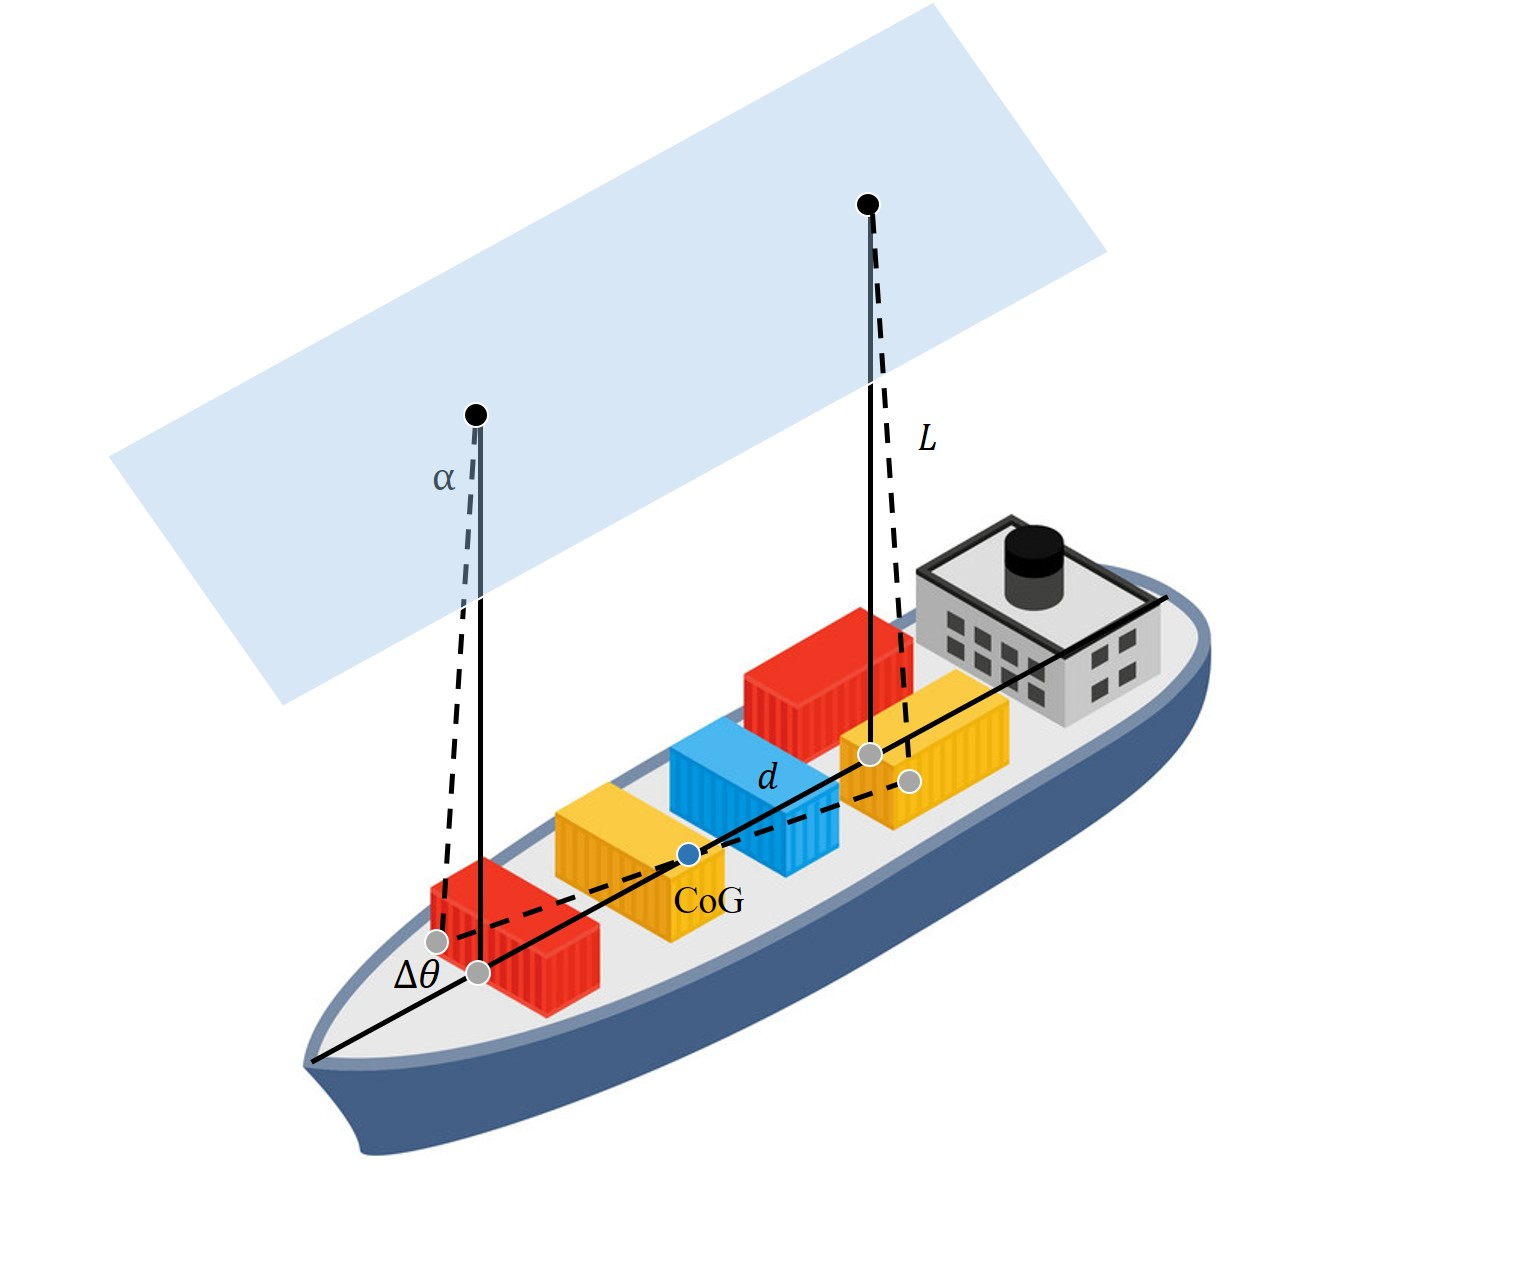
\includegraphics[width=14cm]{chapter01/InertialMeasurement.jpg}
  \bicaption[转动惯量的测量原理]
    {转动惯量的测量原理}
    {Sketch of Inertial Measurement}
  \label{fig:InertialMeasurement}
\end{figure}


\subsection{质量}
重心坐标一般相对于$o_b$
